\begin{figure}
  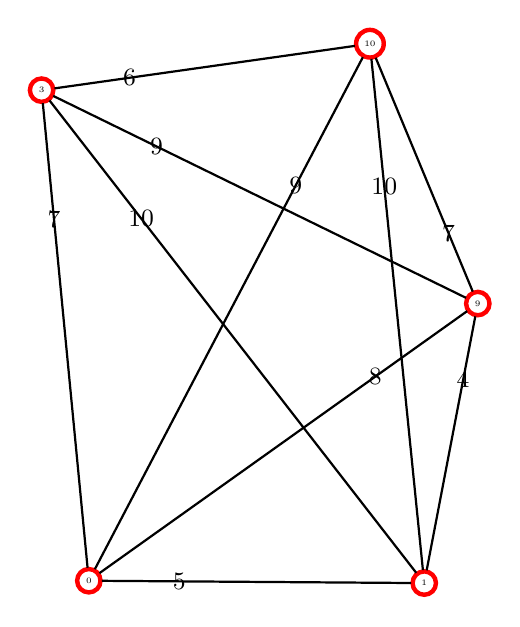
\begin{tikzpicture}[scale=10, ultra thick, node_style/.style={circle,draw=blue,fill=blue!20!,scale=0.6,font=\tiny},terminal_style/.style={circle,draw=red,fill=white,scale=0.6,font=\tiny},edge_style/.style={draw=black, thick,font=\small},selected_edge_style/.style={draw=red, thick, font=\small}]
      \draw
        (0.191, 0.669) node[terminal_style] (3){3}
        (0.745, 0.398) node[terminal_style] (9){9}
        (0.608, 0.728) node[terminal_style] (10){10}
        (0.251, 0.046) node[terminal_style] (0){0}
        (0.677, 0.043) node[terminal_style] (1){1};
      \begin{scope}[-]
        \draw[edge_style] (3) to node[near start] {9} (9);
        \draw[edge_style] (3) to node[near start] {6} (10);
        \draw[edge_style] (3) to node[near start] {7} (0);
        \draw[edge_style] (3) to node[near start] {10} (1);
        \draw[edge_style] (9) to node[near start] {7} (10);
        \draw[edge_style] (9) to node[near start] {8} (0);
        \draw[edge_style] (9) to node[near start] {4} (1);
        \draw[edge_style] (10) to node[near start] {9} (0);
        \draw[edge_style] (10) to node[near start] {10} (1);
        \draw[edge_style] (0) to node[near start] {5} (1);
      \end{scope}
    \end{tikzpicture}
  \caption{test}\label{fig:soln}
\end{figure}